\section{Tuesday, August 6}

\todaybox{We will discuss how to use complex integration to find some real, improper integrals.}

Now that we have a handle on how to integrate complex functions along closed curves, let's see one use for it. A surprising use is that with a bit of creativity we can compute improper integrals:

$$\int_{-\infty}^\infty f(x)dx$$

\noin for a surprising array of functions. Today, we'll see how to do this for rational functions.

To begin, let's remind ourselves what this improper integral means:

\begin{defbo}{Improper Integrals}{} Suppose $f(x)$ is continuous on $\R$. Then the improper integral $\int_{-\infty}^\infty f(x)dx$ is defined to be:

$$\int_{-\infty}^\infty f(x)dx = \lim_{r\rightarrow \infty} \int_{a}^r f(x)dx + \lim_{s\rightarrow -\infty} \int_s^a f(x)dx$$

\noin for any $a\in \R$, and whenever both limits exist. If both limits converge, we say the improper integral converges.\end{defbo}

We won't be working with two limits. For our purposes, we need one limit: $\lim_{r\rightarrow \infty} \int_{-r}^r f(x)dx$. Thankfully, if the integral converges then:

$$\int_{-\infty}^\infty f(x)dx = \lim_{r\rightarrow \infty} \int_{-r}^r f(x)dx$$

This limit actually has a special name:

\begin{defbo}{Principal Value of an Improper Integral}{}
The principal value $\mathrm{P.V.} \int_{-\infty}^\infty f(x)dx$ is $\lim_{r\rightarrow \infty} \int_{-r}^r f(x)dx$.\end{defbo}

So, to compute the improper integrals we're interested in, we're going to first show the integral exists and then calculate the principal value.

We're interested in rational functions. So we'll handle the general case:

\begin{thmbo}{}{} Suppose $p(z),q(z)$ are polynomials. Then:

\begin{itemize}
\item If $q(x)$ has roots in $\R$ which are not roots of $p(x)$ then $\int_{-\infty}^\infty \frac{p(x)}{q(x)}dx$ diverges.
\item If $\deg p(x) \ge \deg q(x) - 1$, then $\int_{-\infty}^\infty \frac{p(x)}{q(x)}dx$ diverges.
\item If $\deg p(x) \le \deg q(x) - 2$ and $q(x) \ne 0$ for $x\in \R$ , then $\int_{-\infty}^\infty \frac{p(x)}{q(x)}dx$ converges,
\end{itemize}
\end{thmbo}

\begin{proof} In the first two cases, comparing the function to $\frac{1}{x}$ gives the desired divergence.

For the final case, suppose $p(x)$ has real roots $r_1 < \dots < r_n$. Since $\frac{p(x)}{q(x)}$ is continuous on $[r_1,r_n]$, then $\int_{r_1}^{r_n} \frac{p(x)}{q(x)}dx$ exists. So we only need to handle the two tails.

By the intermediate value theorem, $\frac{p(x)}{q(x)}$ is either always positive or always negative on each of the intervals $(-\infty,r_1]$ and $[r_n,\infty)$. So we can apply the limit comparison test. In particular, $\lim_{x\rightarrow \pm \infty} \frac{\frac{p(x)}{q(x)}}{\frac{1}{x^2 + 1}}$ exists.

And since $\int_{-\infty}^\infty \frac{1}{x^2 + 1}dx = \pi$, the limit comparison test gives us that $\int_{-\infty}^{r_1} \frac{p(x)}{q(x)}dx$ and $\int_{r_n}^\infty \frac{p(x)}{q(x)}dx$ also exist.
\end{proof}

So now we know that the integrals we care about exist, how do we actually compute the integral?

\begin{ex}{}{} Find $\int_{-\infty}^\infty \frac{x + 1}{x^4+ 2x^2 + 1}dx$.

By our theorem, this integral exists. We need to somehow turn this real integral into a complex one.

We're interested in $\int_{-r}^r \frac{x+1}{x^4 + 2x^2 + 1}dx$. To get a closed curve in $\C$, we look at:

\begin{center}
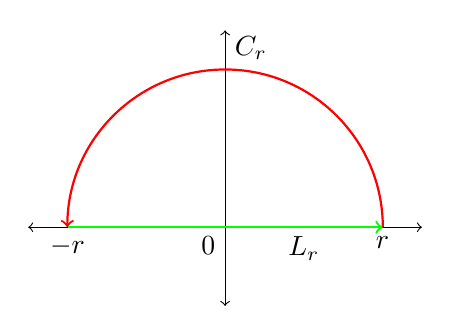
\begin{tikzpicture}

\draw[black, <->] (-2.5,0)--(2.5,0);
\draw[black, <->] (0,-1)--(0,2.5);

\draw[red, ->, thick] ([shift = (0:57pt)] 0,0) arc (0:180:57pt);

\draw[green, ->, thick] (-2,0) -- (2,0);


\draw (0,2) node[above right] {$C_{r}$};

\draw (1,0) node[below] {$L_r$};
\draw (0,0) node[below left] {$0$};
\draw (2,0) node[below] {$r$};
\draw (-2,0) node[below] {$-r$};
\end{tikzpicture}
\end{center}

If $f(z) = \frac{z+1}{z^4 + 2z^2 + 1}$, then the integral we care about is:

$$\int_{-\infty}^\infty f(x)dx = \lim_{r\rightarrow \infty} \int_{-r}^r f(x)dx = \lim_{r\rightarrow \infty} \int_{L_r}f(z)dz$$

To compute this, we'll proceed in three steps:

\begin{enumerate}
\item Show that $\lim_{r\rightarrow \infty} \int_{C_r} f(z)dz = 0$.
\item Show that $\int_{-\infty}^\infty f(z)dz = \lim_{r\rightarrow \infty} \int_{L_r + C_r} f(z)dz$.
\item Compute $\lim_{r\rightarrow \infty} \int_{L_r + C_r} f(z)dz$.
\end{enumerate}

\paragraph{Step 1.} To do this, we'll use M-L estimation (\ref{thm:mlest}). Since $C_r$ is a semicircle of radius $r$, it has length $L = \pi r$.

So we need to estimate the maximum of $|f(z)|$ on $C_r$. Since $f(z) = \frac{z+1}{z^4 + 2z^2 + 1}$, we can get an upper bound for $|f(z)|$ by getting an upper bound for $|z^2|$ and a lower bound for $|z^4 + 2z^2 + 1|$.

By the triangule inequality, $|z+1| \le |z| + 1$. Since $z$ is on $C_r$, $|z| = r$. So $|z+1| \le r+1$.

Also, by a variation of the triangle inequality (specifically that $|a-b| \ge ||a|-|b|$), we see that $|z^4+2z^2+1| \ge r^4 - 2z^2 - 1$ for $r$ large enough (bigger than 2 should be enough.)

Putting these two bounds together, we see that $|f(z)| \le \frac{r+1}{r^4 - 2r^2 - 1}$. And so, M-L esitmation gives us that:

$$\left| \int_{C_r} f(z)dz \right| \le \frac{\pi r(r+1)}{r^4 - 2r^2 -1}$$.

So, in the limit:

$$0 \le \lim_{r\rightarrow \infty} \left| \int_{C_r} f(z)dz \right| \le \lim_{r\rightarrow \infty}\frac{\pi r(r+1)}{r^4 - 2r^2 -1} = 0$$

And so $\lim_{r\rightarrow \infty} \int_{C_r} f(z)dz = 0$.

\paragraph{Step 2:} We know that:

$$\int_{-\infty}^\infty f(x)dx = \lim_{r\rightarrow \infty} \int_{L_r}f(z)dz$$

But since $ \lim_{r\rightarrow \infty} \int_{C_r}f(z)dz = 0$, we have that:

$$\int_{-\infty}^\infty f(x)dx = \lim_{r\rightarrow \infty} \int_{L_r}f(z)dz + \lim_{r\rightarrow \infty} \int_{C_r}f(z)dz =\lim_{r\rightarrow \infty} \int_{L_r+C_r}f(z)dz$$

\noin which is what we wanted to show.

\paragraph{Step 3:} We compute this integral using the residue theorem. Since $z^4+2z^2 + 1 = (z^2+1)^2$, we see that $f(z)$ has two double poles: $\pm i$. Of these, only $i$ is inside the curve (when $r > 1$). As such, when $r > 1$ the residue theorem gives:

$$\int_{L_r + C_R} f(z)dz = 2\pi i \Res\left(\frac{z+1}{z^4+2z^2 +1}; i\right)$$

Since this is a double pole, we compute:

\begin{align*}\Res\left(\frac{z+1}{z^4+2z^2 +1}; i\right) &= \lim_{z\rightarrow i} \frac{d}{d\,z} \frac{(z-i)^2(z+1)}{(z^2+1)^2}\\
&= \lim_{z\rightarrow i} \frac{d}{d\,z} \frac{z+1}{(z+i)^2}\\
&= \lim_{z\rightarrow i} \frac{(z+i)^2 -2(z+i)(z+i)}{(z+i)^4}\\
&=\frac{(2i)^2 - 2(2i)(i+1)}{(2i)^4}\\
&= \frac{-4 +4 -4i}{16}\\
&= \frac{-i}{4}
\end{align*}

And so, all together:

$$\int_{-\infty}^\infty f(x)dx = \lim_{r\rightarrow \infty} \int_{L_r+C_r}f(z)dz = 2\pi i\frac{-i}{4} = \frac{\pi}{2}$$

\end{ex}

For other rational functions, the procedure is identical.